\chapter{Pics应用图片到路径上}
在\tikzname 中可以用\texinline{\tikzset{picname/.pic={tikz
			code}}}来保存一个图形,然后可以在其他绘图语句中用类似于节点的方法来引用(其实是重复绘制)。

\begin{texlst}
	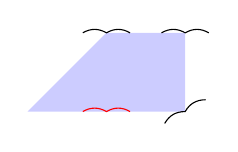
\begin{tikzpicture}
		\tikzset{seagull/.pic={\draw (-3mm, 0) to [bend left] (0,0) to[bend left] (3mm, 0);}}

		\fill[fill=blue!20]
		(1,1)
		-- (2,2) pic {seagull}
		-- (3,2) pic {seagull}
		-- (3,1) pic[rotate=30] {seagull}
		-- (2,1) pic[red] {seagull};
	\end{tikzpicture}
\end{texlst}

与\texinline{node}类似,\texinline{pic}可以用\texinline{transform
	shape}、\texinline{pos}等选项,实现与\texinline{node}类似的效果。

\section{pics/code}
\begin{texlst}
	\begin{tikzpicture}
		\pic [pics/code={\draw (-3mm,0) to [bend left] (0,0) to[bend left] (3mm,0);}] {};
	\end{tikzpicture}
\end{texlst}
如上例所示,\texinline{pic}的代码可以写在选项里面。还可以用如下的写法:
\begin{texlst}
	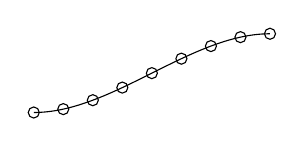
\begin{tikzpicture}
		\draw (0,0) .. controls(1,0) and (2,1) .. (3,1)
		foreach \t in {0, 0.125, ..., 1} {
				pic [pos=\t] {code={\draw circle [radius=2pt];}}};
	\end{tikzpicture}
\end{texlst}

\section{pic actions}
\begin{texlst}
	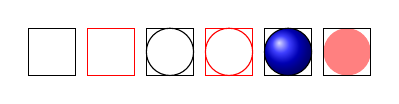
\begin{tikzpicture}
		\tikzset{
			my pic/.pic = {
					\path [pic actions] (0,0) circle[radius=3mm];
					\draw (-3mm, -3mm) rectangle (3mm, 3mm);
				}}

		\pic {my pic} ;
		\pic[red, xshift=0.75cm] {my pic} ;
		\pic[draw, xshift=1.5cm] {my pic} ;
		\pic[draw, red, xshift=2.25cm] {my pic} ;
		\pic[draw, shading=ball, xshift=3cm] {my pic} ;
		\pic[fill=red!50, xshift=3.75cm] {my pic} ;
	\end{tikzpicture}
\end{texlst}

如上例所示,actions可以使用各种绘图的选项。

\section{behind path和in front of path}
与节点类似,\texinline{pic}也有相应的设置在路径之后或之前。
另外还有\texinline{foreground code}与\\\texinline{background code}选项来对应相应的绘制代码。

\section{every pic}
对所有\texinline{pic}设置属性。

\section{name prefix}
如题

\section{pic text 和 pic text options}
如题

\section{Quotes}
\begin{texlst}
	\begin{tikzpicture}
		\draw (3,0) coordinate (A)
		-- (0,1) coordinate (B)
		-- (1,2) coordinate (C)
		pic [draw, "$\alpha$"] {angle};
	\end{tikzpicture}
\end{texlst}
可以用\texinline{every pic quotes}来设置所有\texinline{pic quotes}的属性。

\section{定义新图片样式}
\begin{texlst}
	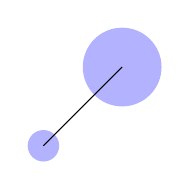
\begin{tikzpicture}[fill=blue!30]
		\tikzset{
			pics/my circle/.style = {
					background code = {\fill circle [radius=#1];}
				}
		}
		\draw (0,0) pic {my circle=2mm} -- (1,1) pic {my circle=5mm};
	\end{tikzpicture}
\end{texlst}
